% Bulk-boundary anomaly inflow: disk geometry with chiral edge mode
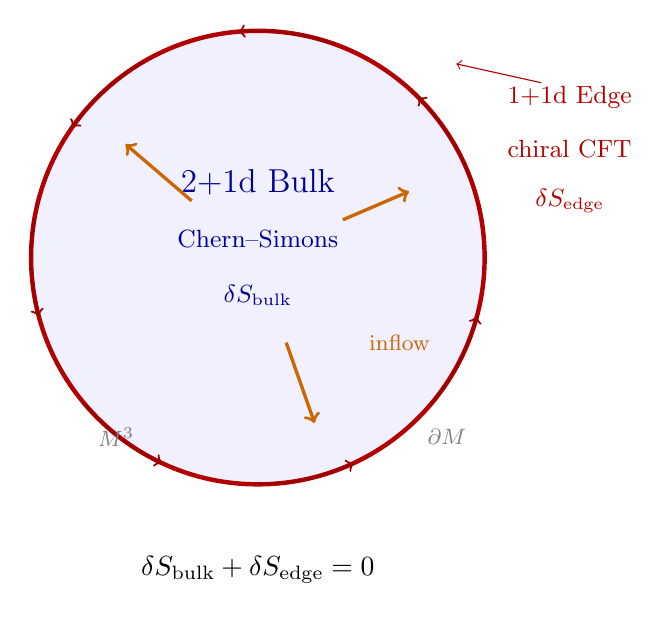
\begin{tikzpicture}[scale=1.2, thick]

  % 2+1d Bulk disk (shaded)
  \fill[blue!6] (0,0) circle (2.4);
  \draw[blue!40!black, thick] (0,0) circle (2.4);

  % 1+1d Boundary edge (highlighted circle)
  \draw[red!70!black, ultra thick] (0,0) circle (2.4);

  % Chiral edge mode arrows (counterclockwise propagation)
  \foreach \angle in {20, 70, 120, 170, 220, 270, 320} {
    \draw[->, red!60!black, thick]
      ({2.4*cos(\angle)}, {2.4*sin(\angle)})
      arc[start angle=\angle, end angle=\angle+25, radius=2.4];
  }

  % Bulk labels
  \node[blue!60!black, font=\large] at (0, 0.8) {$2{+}1$d Bulk};
  \node[blue!60!black, font=\small] at (0, 0.2) {Chern--Simons};
  \node[blue!60!black, font=\small] at (0, -0.4) {$\delta S_{\mathrm{bulk}}$};

  % Inflow arrows (radial, pointing outward toward boundary)
  \draw[->, orange!80!black, very thick] (0.3, -0.9) -- (0.6, -1.75);
  \draw[->, orange!80!black, very thick] (-0.7, 0.6) -- (-1.4, 1.2);
  \draw[->, orange!80!black, very thick] (0.9, 0.4) -- (1.6, 0.7);
  \node[orange!80!black, font=\footnotesize] at (1.5, -0.9) {inflow};

  % Edge/boundary label
  \node[red!70!black, font=\small] at (3.3, 1.7)
    {$1{+}1$d Edge};
  \node[red!70!black, font=\small] at (3.3, 1.15)
    {chiral CFT};
  \node[red!70!black, font=\small] at (3.3, 0.6)
    {$\delta S_{\mathrm{edge}}$};
  \draw[red!70!black, thin, ->] (3.0, 1.85) -- (2.1, 2.05);

  % Cancellation equation
  \node[font=\normalsize] at (0, -3.3)
    {$\delta S_{\mathrm{bulk}} + \delta S_{\mathrm{edge}} = 0$};

  % Dimension annotations
  \node[font=\footnotesize, gray] at (-1.5, -1.9) {$M^3$};
  \node[font=\footnotesize, gray] at (2.0, -1.9) {$\partial M$};

\end{tikzpicture}
